\section{Resultados}


\begin{frame}

    \frametitle{Simulação: Desvio de Obstáculo}

    \begin{columns}[c]

        \begin{column}{0.48\textwidth}
            \centering
            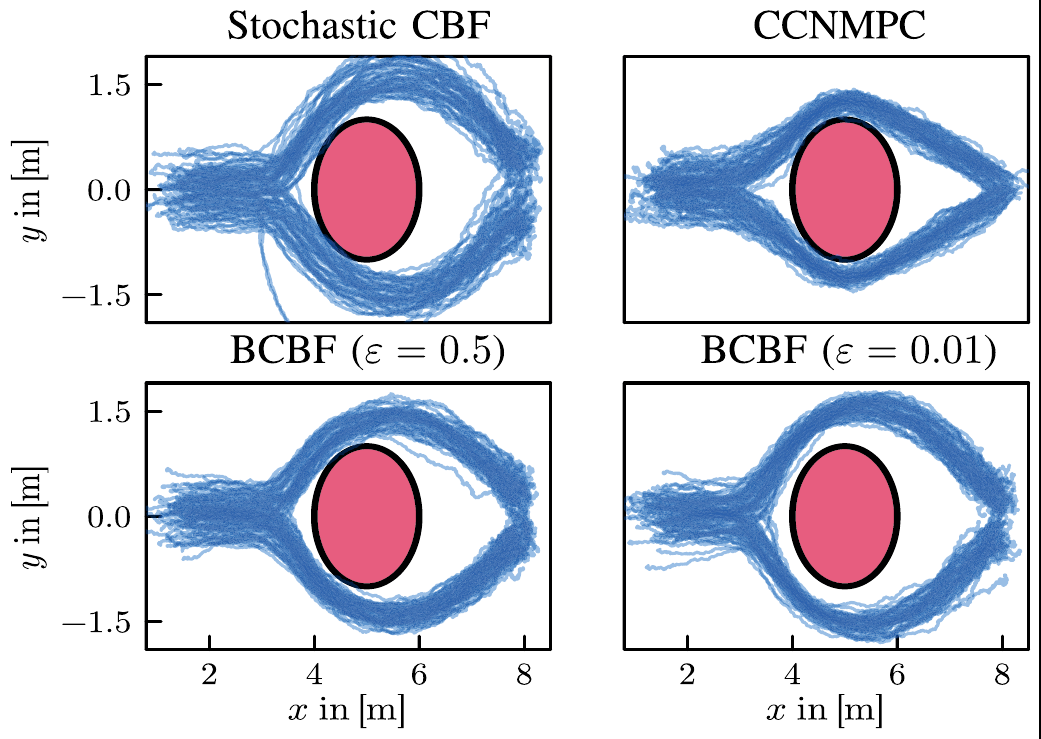
\includegraphics[width=\textwidth]{imagens/fig4_simulation}

            {\tiny 100 trajetórias de um uniciclo ruidoso. Fonte: \citeonline{vahs2023bcbf}.}
        \end{column}

        \begin{column}{0.5\textwidth}
            \centering
            \footnotesize
            \begin{tabular}{lccc}
                \toprule
                & \textbf{CBF estoc.} & \textbf{CCNMPC} & \textbf{BCBF} \\
                \midrule
                Colisões & 3 & 3 & \textbf{0} \\
                Tempo [ms] & 0,8 & 350 & 1,7 \\
                \bottomrule
            \end{tabular}

            {\tiny BCBF com $\varepsilon = 0{,}01$. Adaptado de \citeonline{vahs2023bcbf}.}

            \vspace{3mm}

            \raggedright
            \begin{itemize}
                \item BCBF: \textbf{nenhuma colisão}.
                \item $\sim$200$\times$ mais rápido que o MPC com restrições de chance.
                \item Custo: trajetórias menos eficientes que as do MPC, pois a CBF é reativa.
            \end{itemize}
        \end{column}

    \end{columns}

\end{frame}


\begin{frame}

    \frametitle{Experimento Real: Quadrotor em um Corredor}

    \begin{columns}[c]

        \begin{column}{0.4\textwidth}
            \begin{itemize}
                \item Crazyflie 2.1 com ruído e taxa de medição que \textbf{mudam} ao longo do corredor.
                \item CBF na média do estado: \alert{viola} a segurança.
                \item BCBF: \textbf{20 de 20 execuções seguras}.
                \item BCBF evita o trecho estreito (risco alto demais) e contorna pela esquerda.
            \end{itemize}
        \end{column}

        \begin{column}{0.58\textwidth}
            \centering
            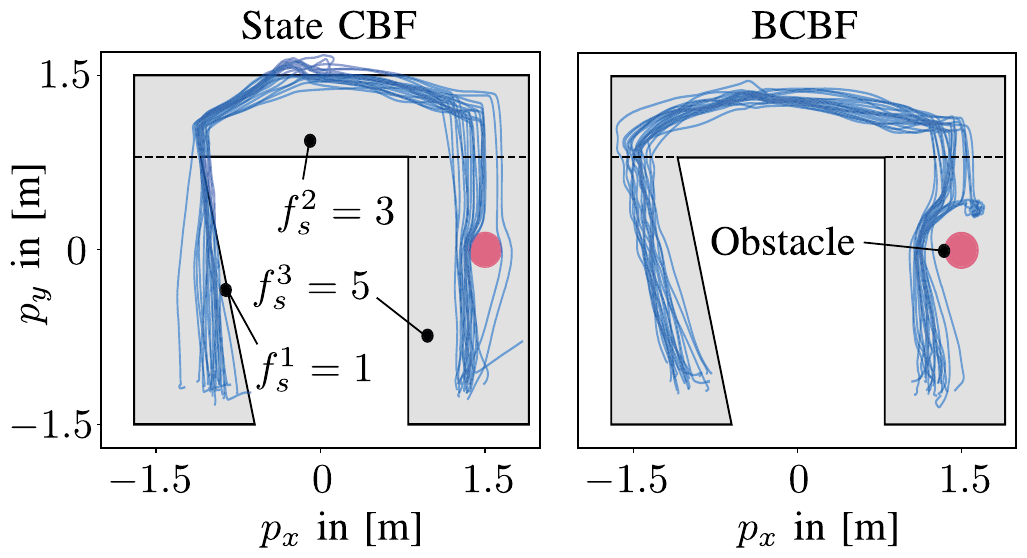
\includegraphics[width=\textwidth]{imagens/fig5_corridor}

            {\tiny Fonte: \citeonline{vahs2023bcbf}.}
        \end{column}

    \end{columns}

\end{frame}
